\documentclass[11pt]{article}
\usepackage[margin=1in]{geometry}
\usepackage{amsmath,amssymb,booktabs,graphicx}
\usepackage[hidelinks]{hyperref}
\usepackage{xurl}
\hypersetup{pdftitle={AFTER: Digital Twins for Cyberattack and Recovery Monitoring in Industrial Robots},pdfauthor={Muhammad Usman; Haiqa Mushtaq},pdfsubject={Synthetic evaluation of alarm recovery under motion-model mismatch}}
\DeclareMathSizes{10}{10}{8}{6}
\setlength{\emergencystretch}{2em}
\setlength{\textfloatsep}{18pt plus 2pt minus 2pt}
\newtheorem{proposition}{Proposition}
\newenvironment{proof}{\par\noindent\textit{Proof.}\ }{\hfill\textit{Q.E.D.}\par}
\title{AFTER: Digital Twins for Cyberattack and Recovery Monitoring in Industrial Robots}
\author{Muhammad Usman \and Haiqa Mushtaq}
\date{}
\begin{document}
\maketitle
\begin{abstract}
Cyberattack detection and alarm clearance impose different demands on a robotic digital twin. A predictor may follow unauthorized motion and lose evidence of its persistence, while an inaccurate reference may prevent clearance after the plant has recovered. We examine this tension through a same-plant counterfactual recovery target, a frozen comparison of thirteen monitoring rules, and a subsequent normal-only reference-development study. The attack evaluation comprises 216 synthetic episodes covering command corruption, legitimate changes, missing command context and three plant configurations. Adding an empirical uncertainty allowance reduced benign alarm observations from 621 to 309 relative to nominal fixed return, but permitted timely clearance in only 36 of 108 detected events with physical return. At the same entry threshold, removing that allowance yielded 140 benign alarm observations and 108 timely clearances without observed premature clearing. A finite search over 63 clean-data models then reduced the allowance by 51.27\% and 38.56\% on the two more difficult plants, yet the overall normal-operation feasibility requirement still failed. A conditional Gaussian calculation explains why: combining a maximum noisy calibration residual with a new instantaneous discrepancy can exhaust the return tolerance even with a perfect reference. The results identify a concrete limitation of the tested clearance design and establish normal-operation feasibility as a necessary check before interpreting reduced alarm burden as improved recovery.
\end{abstract}
\noindent\textbf{Keywords:} digital twins; industrial robots; cyberattack detection; alarm clearance; system identification; model mismatch.

\section{Introduction}
A robot can continue to move away from its intended trajectory after a corrupted command has been removed. An alarm that clears at command restoration can therefore disappear before the physical effect ends. The reverse problem also occurs: an accurate account of the robot's recovery may remain inconsistent with an inaccurate nominal model, leaving an alarm active after normal motion resumes. Both errors matter when a digital twin supplies evidence for cyberattack monitoring.

Recent robotic anomaly detectors use motion measurements to identify departures from expected behavior~\cite{casper,edge}. Hybrid twins combine models of robot mechanics, drives and control with learned components~\cite{hybrid}. These approaches motivate a closer examination of the relationship between prediction quality and alarm recovery. A small one-step prediction error need not indicate a return to authorized motion, because the predictor may already be following the deviation. Conversely, a large free-reference error can reflect ordinary model mismatch rather than a continuing attack.

We study a specific question: \emph{under model mismatch, when does discrepancy from a command-driven reference provide usable evidence for clearing a robotic attack alarm?} The monitor receives noisy joint positions and velocities together with a protected record of approved commands. An attacker can corrupt the downstream command path. This information model permits a reference to predict authorized motion while preserving a distinction between approved and executed commands.

Our investigation has two empirical stages. First, a prospectively frozen attack evaluation compares thirteen detection and clearance rules under common observations. Second, prompted by the first stage's failure, a separately specified normal-only study tests whether better clean-data identification restores clearance feasibility. The second stage does not retrospectively improve the attack results. A subsequent analytical diagnostic isolates the effect of measurement noise on the same clearance inequality.

The paper contributes an explicit separation of physical return from nominal-reference proximity; a complete comparison showing how an uncertainty allowance can obstruct recovery despite fewer benign alarms; and a matched normal-model study that distinguishes improved prediction from a usable return margin. The conditional bounds and noise calculation explain the observed obstruction. They use established interval and probability arguments, and the evidence does not establish a new detector that outperforms the recent literature.

\section{Related work}
\subsection{Robotic anomaly detection and digital twins}
CASPER detects anomalous industrial-arm motion using external inertial sensing and contextual information~\cite{casper}. Its edge-computing successor develops real-time robotic anomaly detection~\cite{edge}. These are relevant application baselines, but their sensing modality and experimental protocols differ from the joint-state and approved-command simulation in this paper. We do not transfer their published scores or label our common-input controls as faithful reproductions of either method.

Ayankoso et al. describe a hybrid twin combining robot kinematic and dynamic models, drive and control information, and learned uncertainty accommodation for collaborative-robot condition monitoring~\cite{hybrid}. This establishes the relevance of model fidelity and uncertainty to robotic twins. It does not establish that an uncertainty allowance improves attack-alarm clearance. More broadly, Classens et al. develop recursive identification of structured mechanical systems through instrumental variables and block-coordinate descent~\cite{identification}. Our fixed ARX/FIR search is an ordinary identification exercise rather than an alternative claim to that contribution.

\subsection{Uncertainty, runtime monitoring and recovery}
FAIL-Detect learns or constructs scalar signals and calibrates uncertainty-aware failure monitors from successful robot rollouts~\cite{fail}. Its full system concerns imitation-learning policies and includes signal-learning and calibration choices absent from our experiment. We independently implement a restricted constant episode-band component on our shared discrepancy signal. We therefore compare a thresholding principle under common inputs, not the full published method.

Interval-observer fault detection explicitly considers the effect of uncertain models and observer design~\cite{interval}. Adding a bound to a measured residual, or requiring a dwell period before clearing an alarm, is not by itself a new digital-twin mechanism. The useful question here is whether the resulting decision remains feasible at the tolerance required by the recovery definition.

The RESCUE preprint evaluates the value of runtime alarms through counterfactual robot-policy interventions~\cite{rescue}. It shows why detection accuracy and intervention usefulness must be distinguished. Our evaluator instead compares corrupted and uncorrupted executions of the same plant to measure the disappearance of a motion deviation. The overlap is substantive: counterfactual evaluation is existing methodology. Our narrower emphasis is the interaction among reference error, sensor noise and a particular alarm-clearance rule. The experiments support conclusions about this rule and these simulated conditions, rather than a ranking against complete recent robotic-security systems.

\section{Recovery target and clearance feasibility}
\subsection{What the monitor observes}
Let $x_t=(q_1,q_2,\dot q_1,\dot q_2)$ denote the actual state and $x_t^0$ the state of the same plant under the complete approved command history without corruption. The monitor receives $y_t=x_t+n_t$, approved commands $u_t$, and their availability indicator. A reference $r_t$ predicts the authorized trajectory. Positive scales $s_j$ are estimated from clean training observations only. Define
\begin{equation}
 \|v\|_s=\max_j |v_j|/s_j,\qquad
 d_t=\|x_t-x_t^0\|_s,\qquad c_t=\|y_t-r_t\|_s.
 \label{eq:discrepancies}
\end{equation}
The evaluator computes $d_t$; the monitor computes $c_t$. In the noise-free case, $x_t=r_t\ne x_t^0$ can give $c_t=0$ with $d_t>0$. Similarly, $x_t=x_t^0\ne r_t$ gives $d_t=0$ with $c_t>0$. A reference-discrepancy threshold consequently requires an assumption linking $r_t$ to $x_t^0$ before it can represent physical return.

\subsection{Conditional error bounds}
\begin{proposition}
If $\|x_t^0-r_t\|_s\le b_t$ and $\|n_t\|_s\le\eta_t$, then
\begin{equation}
 \max(0,c_t-b_t-\eta_t)\le d_t\le c_t+b_t+\eta_t.
 \label{eq:bound}
\end{equation}
\end{proposition}
\begin{proof}
Write $x_t-x_t^0=(y_t-r_t)-n_t-(x_t^0-r_t)$ and apply the triangle and reverse triangle inequalities. Aligned scalar errors attain the extremes, so scalar allowances alone do not generally permit tighter bounds.
\end{proof}

A sufficient return condition at tolerance $\delta$ is $c_t+b_t+\eta_t\le\delta$. This gives a simple feasibility test before any alarm experiment.
\begin{proposition}
Suppose reference and measurement errors lie in coordinate boxes with half-widths $b_{t,j}$ and $\eta_{t,j}$. Return within $\delta$ holds for every pair in those boxes exactly when
\begin{equation}
 \max_j\frac{|y_{t,j}-r_{t,j}|+b_{t,j}+\eta_{t,j}}{s_j}\le\delta.
 \label{eq:box}
\end{equation}
If $b_{t,j}+\eta_{t,j}>\delta s_j$ in any coordinate, no observation can satisfy this condition.
\end{proposition}
\begin{proof}
In each coordinate, the two admissible errors can align against the measured displacement. Their summed magnitude attains the triangle-inequality bound. The observed absolute displacement is nonnegative, yielding the infeasibility statement.
\end{proof}

These statements are conditional geometric facts. The simulated sensors have unbounded Gaussian noise, and the experiment uses an empirical discrepancy allowance rather than a verified deterministic enclosure. Specifically, the tested rule requires $c_t+b\le\delta$, where $b$ is the largest observed normal discrepancy. It is a heuristic motivated by the upper-bound form, not an implementation of a proven safety certificate. Because $b$ contains both model error and noise, interpreting it as pure reference uncertainty would be incorrect. A dwell period cannot restore feasibility when $b>\delta$.

\section{Simulation and threat model}
\subsection{Plant, controller and sensing}
All evaluation observations are synthetic. The plant is a horizontal two-joint point-mass arm governed by
\begin{equation}
 M(q)\ddot q+C(q,\dot q)+B\dot q=\tau.
\end{equation}
Writing $a=m_2l_1l_2$ and $d=m_2l_2^2$,
\begin{align}
 M(q)&=\begin{bmatrix}(m_1+m_2)l_1^2+d+2a\cos q_2&d+a\cos q_2\\d+a\cos q_2&d\end{bmatrix},\\
 C(q,\dot q)&=a\sin q_2\begin{bmatrix}-2\dot q_1\dot q_2-\dot q_2^2\\\dot q_1^2\end{bmatrix}.
\end{align}
A PD controller requests componentwise saturated torque
\begin{equation}
 \tau^*=\operatorname{clip}\{K_p(q^c-q)+K_d(\dot q^c-\dot q),-20,20\},
\end{equation}
with $K_p=\operatorname{diag}(18,12)$ and $K_d=\operatorname{diag}(4,3)$. Where actuator lag is present, $\dot\tau=(\tau^*-\tau)/T_a$. Nominal masses are $(1,0.8)$ kg, lengths $(0.5,0.4)$ m, and damping coefficients $(0.08,0.06)$. The nominal physics reference retains these parameters; Table~\ref{tab:plants} specifies the actual plants.

\begin{table}[htbp]\centering\small
\caption{Simulated plant configurations. Mass and damping entries multiply the nominal values; noise multiplies the stated sensor standard deviations.}\label{tab:plants}
\setlength{\tabcolsep}{5pt}
\begin{tabular}{lcccrr}\toprule
Plant & Mass factors & Damping factors & Lengths (m) & Lag (s) & Noise\\\midrule
Q1 & (1.10,0.86) & (0.80,1.20) & (0.48,0.42) & 0 & 1.0\\
Q2 & (0.88,1.15) & (1.30,0.85) & (0.53,0.37) & 0.03 & 1.0\\
Q3 & (1.16,1.06) & (0.90,1.40) & (0.46,0.43) & 0.06 & 1.5\\\bottomrule
\end{tabular}
\end{table}

Position and velocity noise are independent zero-mean Gaussians with standard deviations 0.0005 rad and 0.002 rad/s, respectively, before the plant multiplier. Episodes contain 1,200 observations at 50 Hz. Fourth-order Runge--Kutta integration uses eight substeps per observation. A short lagged trajectory was checked against a separate SciPy integration. This verifies numerical consistency; the model excludes gravity, contact, flexibility and thermal effects and has not been validated against physical robot measurements.

\subsection{Adversary and information boundaries}
The attacker changes executed commands downstream of the protected approved-command record. It can impose an offset, slow progression or hold a command. Joint measurements remain truthful apart from the declared sensor noise. Legitimate task changes update both command paths. The monitor receives no intervention labels, true state, actual plant parameters or paired counterfactual trajectory in its calculations.

The attack-study implementation passes a complete episode dictionary to the monitoring routine. Source inspection and three restricted-input replays support the stated input use, but this is not an enforced isolation boundary. The later normal-only study uses a restricted observation type. Neither study addresses joint compromise of sensing and approved commands, poisoned commissioning, or attribution of malicious intent from motion alone.

Missing approved commands invalidate the complete history required by a free reference. Command-dependent methods therefore remain unknown for the rest of that episode, even after availability resumes. Unknown intervals remain in coverage and missed-event accounting; they are not silently removed from the evaluation population. Persistence does not require commands.

\section{Study I: attack detection and recovery}
\subsection{Clean commissioning and model state}
Each plant provides three known-clean commissioning episodes. Their eligible observations define the channel means and population standard deviations. Let $z_t=(y_t-\mu)/s$ denote standardized state. The ARX reference predicts
\begin{equation}
 \widehat z_t=a_0+\sum_{k=1}^{p}A_k\widetilde z_{t-k}
                    +\sum_{k=1}^{p}D_k u_{t-k},
 \label{eq:arx}
\end{equation}
where the four-component command contains approved position and velocity. For the free reference, $\widetilde z$ is its own predicted state after initialization. The one-step control instead uses measured state history. Thus the reference's maintained state is its lagged trajectory; its command-driven recurrence makes prospective predictions, while synchronization is restricted to the initial observed prefix. The following observer provides a separate measurement-corrected comparison.

Study I fixes $p=4$ and fits a ridge of $10^{-7}$ to mean normal equations, without penalizing the intercept. The first 100 observations are excluded from fitting targets. Homogeneous recursion must have spectral radius below one. The free reference starts from four observed states and receives no subsequent measurement correction. Fitted parameters remain fixed during evaluation.

\subsection{Monitoring rules and calibration}
All scores are maximum absolute standardized discrepancies. The roster includes persistence, one-step ARX, a nominal following observer, nominal free references, and learned free references. The following observer predicts before correcting its state with gains $(0.65,0.65,0.35,0.35)$. Point rules alarm when their score exceeds $h$. Hysteresis enters at the same strict exceedance and clears after ten valid observations at or below $h/2$.

Fixed-return rules instead clear after ten observations with the relevant reference discrepancy at most $\delta=0.1$. The uncertainty-return candidate requires $c_t+b\le0.1$. An entry-threshold exceedance takes priority and resets the clearance counter. Two matched ablations keep the candidate entry threshold while removing $b$ or reducing the dwell from ten samples to one.

Each plant has nineteen normal calibration episodes. Each main rule calibrates its complete alarm state machine to at most 209 alarmed observations among 20,900 eligible observations. The threshold search selects the boundary score satisfying this finite budget. The candidate allowance is the largest learned-reference discrepancy in the same calibration episodes. Calibration uses no attack labels and does not guarantee a future 1\% false-alarm rate.

The additional constant episode band takes the maximum of the nineteen whole-episode discrepancy maxima. Its rank is $\lceil(19+1)(1-0.05)\rceil=19$. This component has a different calibration objective from the main point-alarm budget. The fixed calibration grid and shifted task families do not establish the exchangeability needed for a conformal coverage guarantee. Matched-entry ablations also have their own realized calibration burdens; their role is to isolate components at an identical entry threshold.

\subsection{Frozen evaluation and metrics}
The fresh matrix crosses three new command families, three plants, seeds 17, 42 and 2026, and eight conditions, giving 216 episodes and 2,808 method/episode outcomes. The conditions are unchanged motion, authorized offset, authorized slowdown, brief unauthorized offset, persistent offset, held command, unauthorized slowdown, and offset with missing command context. The first 100 observations are processed but excluded from metrics. Corruption begins at sample 320 and ends before sample 620, except the brief offset, which lasts six samples. Offset magnitude is 0.14 rad on joint 1, slowdown rate is 0.6, and missing context spans $[320,380)$. States do not reset at intervention boundaries.

For evaluation only, a paired simulation uses the same plant and initial state with approved commands throughout. Physical return is the first post-restoration run of ten true-state observations satisfying $d_t\le0.1$, searched over five seconds. Its timestamp is the start of that qualifying window, assigned retrospectively by the evaluator. This tolerance defines a motion-effect diagnostic, not task success, collision avoidance or product quality. Nominal-reference return is retained as a secondary diagnostic.

We report unadjusted precision, recall and F1 against the command-corruption interval, average precision (AP), alarm observations and episodes on wholly benign trajectories, coverage, event overlap, fresh alarm onset, misses, premature clearing and timely clearance after physical return. An alarm already active at intervention onset counts as overlap but not fresh detection. Persistent post-intervention alarms can be false positives under interval labels while still reflecting unrecovered motion; the recovery measures expose this difference. Conditional clearance counts include only detected events with measured physical return, while all misses remain visible.

Premature clearing means an active-to-inactive transition after first detection and before the physical-return timestamp. Timely clearance means a known inactive alarm observation within five seconds of that timestamp, including alarms already inactive when physical return begins. Consequently, the timely-clearance count must be interpreted alongside premature clearing; it does not by itself show that an alarm remained active until recovery.

The predeclared primary criterion combines four requirements: at least 25\% fewer benign alarm observations than nominal fixed return; no additional missed or prematurely cleared events; at least 95\% timely clearances among detected-returned events; and benign burden no more than 10\% above learned-reference hysteresis. Models and thresholds were sealed before evaluation generation, and all score artifacts were sealed before joint outcome computation.

\subsection{Results}
The primary criterion failed. The candidate reduced benign alarm observations from 621 to 309, or 50.24\%, but achieved timely clearance in only 36 of 108 detected-returned events. It overlapped 108 of 135 interventions, with 104 fresh onsets. Table~\ref{tab:attack} retains every method; Figure~\ref{fig:recovery} contrasts its apparent alarm-burden benefit with the clearing failure.

\begin{table}[htbp]\centering\small
\caption{Study I: complete pooled comparison. Benign counts use 89,100 observations. Overlap and fresh onset each use 135 interventions. Early counts events with premature clearing. Clear/return retains the detected-returned denominator. CP and matched-entry rows have distinct calibration interpretations.}\label{tab:attack}
\setlength{\tabcolsep}{4pt}
\begin{tabular}{lrrrrr}\toprule
Method & Benign & F1 & Overlap/fresh & Early & Clear/return \\\midrule
Persistence & 878 & 0.057 & 127/127 & 127 & 127/127 \\
ARX one-step & 792 & 0.803 & 108/108 & 108 & 108/108 \\
Following point & 794 & 0.808 & 108/108 & 108 & 108/108 \\
Following hysteresis & 993 & 0.785 & 108/108 & 108 & 108/108 \\
Nominal hysteresis & 789 & 0.713 & 108/108 & 45 & 108/108 \\
Nominal fixed return & 621 & 0.657 & 108/108 & 0 & 108/108 \\
Learned point & 819 & 0.700 & 108/108 & 18 & 108/108 \\
Learned hysteresis & 792 & 0.683 & 108/108 & 0 & 108/108 \\
Learned fixed return & 827 & 0.690 & 108/108 & 0 & 108/108 \\
Uncertainty return & 309 & 0.446 & 108/104 & 0 & 36/108 \\
Episode CP band & 0 & 0.744 & 108/108 & 75 & 108/108 \\
Matched no allowance & 140 & 0.709 & 108/108 & 0 & 108/108 \\
Matched no dwell & 20 & 0.453 & 108/108 & 0 & 36/108 \\
\bottomrule\end{tabular}

\end{table}

\begin{figure}[htbp]\centering
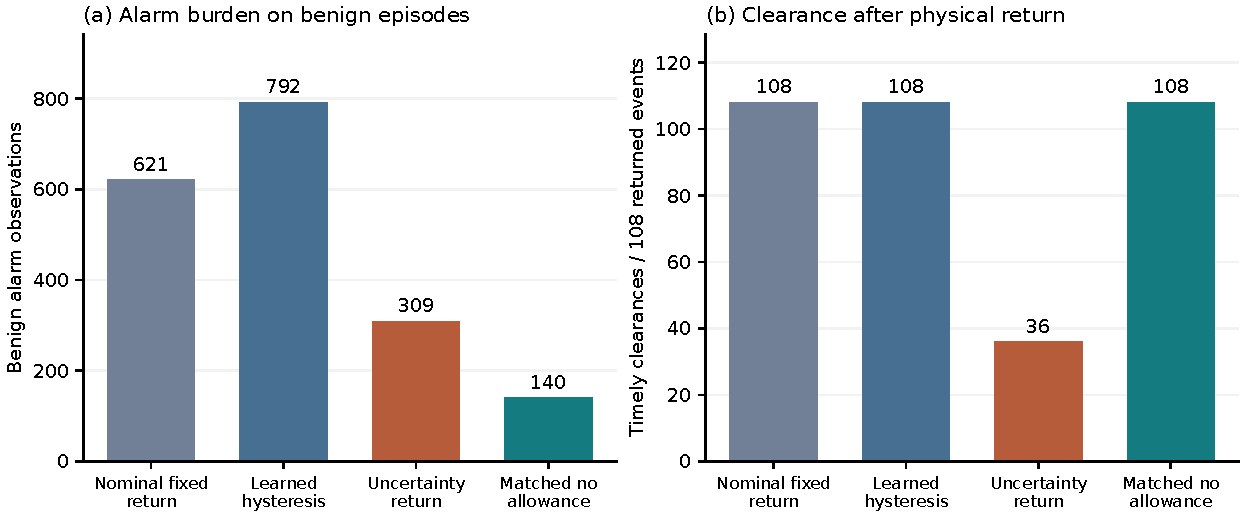
\includegraphics[width=\linewidth]{figures/recovery.pdf}
\caption{Saved Study I outcomes. All four displayed rules have zero observed premature clears, but the uncertainty-return rule fails timely clearance on 72 detected-returned events. Fewer benign alarm observations alone conceal this failure.}\label{fig:recovery}
\end{figure}

The learned-reference spectral radii are 0.95595, 0.96690 and 0.97148 for Q1--Q3. Their empirical allowances are 0.07088, 0.19149 and 0.20928. Thus Q2 and Q3 have $b>\delta$, making clearance mathematically impossible for the tested rule. Their zero benign alarm counts do not demonstrate useful recovery. All 36 timely candidate clearances come from Q1.

Removing the allowance at the same entry threshold reduces benign alarms further, to 140, and restores timely clearance in all 108 detected-returned events. Fresh onsets increase from 104 to 108, with no observed premature clears. Removing dwell alone reduces benign alarms to 20 but leaves the same 72 clearing failures. The matched comparison identifies the allowance as the obstruction; a longer or shorter waiting period cannot remove it.

The following-observer point rule achieves F1 0.808 but clears prematurely in all 108 detected events. The episode band has no benign alarm observations and F1 0.744, yet clears prematurely in 75 events. Learned-reference hysteresis has 792 benign alarms, no premature clears and 108 timely clearances. These outcomes show why interval detection scores and recovery measurements must be read together.

All 27 missing-context interventions are missed by command-dependent methods under the unknown-history rule. Nominal-reference and paired-plant return times differ in 21 of 135 intervention episodes. The empirical allowance encloses the complete eligible counterfactual-reference discrepancy in 189 of 216 episodes, which does not establish a distribution-shift guarantee. Further point metrics, unknown coverage and alarm-episode rates appear in Appendix~\ref{app:metrics}.

\section{Study II: can better commissioning restore feasibility?}
\subsection{Finite normal-only development procedure}
Study II follows Study I and is an outcome-informed diagnosis. It uses the same three clean commissioning episodes per plant but introduces a finite model bank before generating new normal checks. ARX orders $\{4,8,16,32\}$ and FIR lengths $\{16,32,64\}$ each use ridge values $\{10^{-7},10^{-5},10^{-3}\}$. There are 21 fits per plant and 63 in total. All are eligible; no failed candidate is omitted. FIR uses the command-history terms and intercept in Equation~\ref{eq:arx}, without state-history terms.

The nineteen previously used normal calibration episodes are explicitly reused for development: the first nine select a model, the next five estimate its allowance, and the last five provide archived checks. Selection minimizes the worst episode's 99th-percentile discrepancy, breaking ties by mean standardized RMSE, parameter count and model identifier. The allowance is the maximum over the five assigned episodes, or 5,500 observations. The archived checks are not relabeled independent holdouts.

Every reference receives the same 100-observation initialization prefix. A free ARX model uses the last $p$ states of that prefix, then feeds back its predictions. This differs from Study I's four-state initialization and nineteen-episode allowance. We therefore compare selected models to a matched ARX(4) within Study II. Its fitted coefficients and training transformations equal the earlier fit exactly; differences between studies' allowances cannot be attributed solely to model order.

New checks cross three previously ungenerated task families, three plants, three seeds and three normal conditions: unchanged motion, authorized offset and authorized slowdown. This gives 81 new normal episodes. Including fifteen archived checks and six recorded roles gives 576 outcomes. The selected overall model equals the selected ARX on each plant; these duplicate roles are not separate evidence.

\subsection{Feasibility criterion}
For each reference, we measure the fraction of eligible normal observations satisfying $c_t+b\le0.1$. Four diagnostic probes per episode, starting at samples 100, 320, 620 and 900, force an active latch and seek ten qualifying observations within five seconds. These probes ignore alarm-entry priority: they test the opportunity to clear during normal motion, not attack detection or actual post-attack recovery.

The predeclared admission rule requires $b<0.1$, at least 95\% feasible normal observations, and at least 95\% successful probes on every plant. A model can clear every probe yet fail the point-fraction condition. The criterion is retained unchanged after observing the results.

\subsection{Results}
The selected ARX orders are 8, 16 and 32 for Q1, Q2 and Q3, all with ridge $10^{-7}$. Mean standardized RMSE falls from 0.009477 to 0.009337 on Q1, from 0.010203 to 0.009716 on Q2, and from 0.015865 to 0.014388 on Q3. Table~\ref{tab:normal} and Figure~\ref{fig:commissioning} show that these improvements do not establish clearance feasibility across all plants.

\begin{table}[htbp]\centering\small
\caption{Study II: selected ARX versus matched ARX(4). $b_4$ and $b_\star$ are their respective allowances. Feasibility uses 29,700 new normal observations per plant. Each plant has 108 diagnostic probe starts.}\label{tab:normal}
\setlength{\tabcolsep}{4pt}
\begin{tabular}{lrrrrrr}\toprule
Plant & Order & $b_4$ & $b_\star$ & Reduction (\%) & Feasible (\%) & Clear/probes \\\midrule
Q1 & 8 & 0.0553 & 0.0553 & 0.06 & 99.82 & 108/108 \\
Q2 & 16 & 0.1469 & 0.0716 & 51.27 & 93.32 & 108/108 \\
Q3 & 32 & 0.1913 & 0.1175 & 38.56 & 0.00 & 0/108 \\
\bottomrule\end{tabular}

\end{table}

\begin{figure}[htbp]\centering
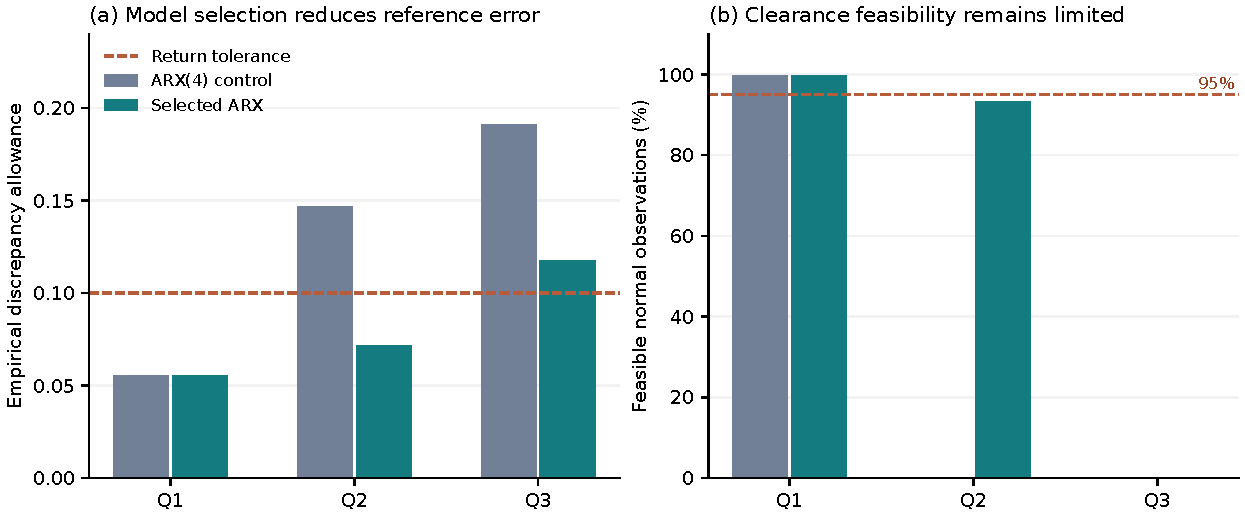
\includegraphics[width=\linewidth]{figures/commissioning.pdf}
\caption{Normal-only model development. Lower discrepancy allowances make Q2's inequality reachable, but its feasible fraction remains below 95\%. Q3's selected allowance still exceeds the return tolerance.}\label{fig:commissioning}
\end{figure}

On Q2, the allowance drops 51.27\%, from 0.146910 to 0.071592. All 108 probes clear, yet only 93.32\% of normal observations satisfy the inequality. Q3 improves by 38.56\%, from 0.191250 to 0.117495, but retains an allowance above the tolerance and clears none of its probes. Only Q1 passes all requirements. FIR(64) is selected within the FIR family on all plants but performs worse in this search. The full role comparison, including one-step ARX and command-as-state controls, is in Appendix~\ref{app:normal}. No attack evaluation of the selected replacements was conducted.

\section{Noise allocation explains the remaining obstruction}
The normal-study outcome motivates a separate post-study calculation. Consider a hypothetical perfect free reference $r_t=x_t^0$ under normal motion, with the simulator's independent Gaussian measurement noise and fixed training scales. Let $\nu_j=\sigma_j/s_j$. The distribution of the scalar noise discrepancy is
\begin{equation}
 F(x)=\Pr\{\|n_t\|_s\le x\}
     =\prod_{j=1}^{4}\operatorname{erf}\!\left(\frac{x}{\sqrt{2}\nu_j}\right),
 \qquad x\ge0.
\end{equation}
For an empirical allowance $B$ equal to the maximum of $N$ independent calibration discrepancies,
\begin{equation}
 \Pr(B\le b)=F(b)^N.
\end{equation}
Conditioned on $B$, a new normal observation satisfies the rule with probability $F(\delta-B)$, taking $F(x)=0$ for $x<0$. A population feasibility of at least $\gamma$ therefore requires
\begin{equation}
 B\le\delta-F^{-1}(\gamma),\qquad
 \Pr\{F(\delta-B)\ge\gamma\}
 =F\!\left(\delta-F^{-1}(\gamma)\right)^N.
 \label{eq:noiseprob}
\end{equation}
This elementary calculation describes allocation of a fixed tolerance between two noisy quantities. Increasing $N$ makes the calibration maximum stochastically larger, even though a larger calibration sample might otherwise seem reassuring. Better reference fitting cannot remove this noise-only contribution.

\begin{table}[htbp]\centering\small
\caption{Conditional perfect-reference diagnostic with $N=5{,}500$, $\delta=0.1$ and $\gamma=0.95$. The final column is the probability that a noise-only calibration maximum leaves enough margin for 95\% population feasibility.}\label{tab:noise}
\begin{tabular}{lrrr}\toprule
Plant & $F^{-1}(0.95)$ & $\delta-F^{-1}(0.95)$ & Margin probability \\\midrule
Q1 & 0.028251 & 0.071749 & 0.999828 \\
Q2 & 0.027914 & 0.072086 & 0.999897 \\
Q3 & 0.041737 & 0.058263 & $2.19\times10^{-9}$ \\
\bottomrule\end{tabular}

\end{table}

For Q3, the single-observation noise quantile is 0.041737, leaving an allowable calibration maximum of only 0.058263. Equation~\ref{eq:noiseprob} gives approximately $2.19\times10^{-9}$. The corresponding probabilities for Q1 and Q2 exceed 0.9998. Two numerical implementations agree on these values.

The calculation conditions on the declared independent Gaussian noise and the fitted training scales. It is a population statement about the clearance inequality, not the probability of passing a finite empirical check, a dwell-time calculation, or an estimate across real robots. It was added after Study II and changed no selected model, tolerance or criterion. It explains why the maximum-plus-discrepancy construction can remain unusable even when reference error is removed; it does not establish that all uncertainty-aware recovery decisions fail.

\section{Discussion}
The studies distinguish three questions that a single detection score cannot answer: whether unauthorized motion is detected, whether its physical effect persists, and whether the chosen clearance rule can recognize normal motion. The candidate's reduced benign alarm count initially appears favorable, but two plants have an unreachable clearing condition. A matched ordinary control removes this obstruction and is stronger on the recorded outcomes. The uncertainty-addition component consequently has no demonstrated benefit here.

Improved commissioning addresses one part of the problem. Longer ARX histories reduce normal prediction error and make Q2's condition reachable. The remaining failure on Q3, together with the perfect-reference calculation, shows that reference bias and measurement noise require separate treatment. A maximum of noisy residuals is not interchangeable with a bound on model error. Once it is added to another noisy residual, the available tolerance can be consumed before any genuine physical deviation is considered.

This suggests a practical design sequence: define the physical return target and trusted information; check the return condition under normal motion; then evaluate detection, persistence and recovery jointly. Algebraic reachability, point feasibility and successful dwell probes provide different evidence. None alone establishes a safe reset policy. Statistical estimation, averaging and noise-aware observers are established tools for revising such a decision, and a replacement would need comparison against those tools rather than a new name for the present combination.

The same-plant counterfactual also changes interpretation. In 21 intervention episodes, nominal-reference and actual-plant return times disagree. Measuring recovery against the detector's own nominal model can conflate model mismatch with remaining attack effects. Simulation permits the two trajectories to be separated exactly within the model. In a physical deployment, the counterfactual would itself be uncertain and would need independent justification.

\subsection{Evidence scope}
The evidence comes from three specified plant configurations in one simulator. Noise seeds repeat a physical condition; they are not independent robot acquisitions. Geometry, damping, lag and noise vary together, preventing causal attribution of a subgroup difference to a single factor. There are no contact-rich tasks, changeovers between manufacturing processes, field attacks or hardware measurements. The observed return tolerance has no established safety interpretation.

The comparison contains common-information controls and a restricted recent calibration component, rather than three full recent paper reproductions. External-IMU baselines cannot be ranked fairly against protected-command monitors without resolving their input and protocol differences. This limits claims of comparative performance, even where the internal ablations are informative.

The two stages also have different evidential roles. Study I prospectively evaluates a fixed candidate; Study II is a separately frozen normal-only response to its failure. The post-study noise calculation explains a mechanism under explicit assumptions. All conditions are now exposed. A redesigned alarm rule evaluated on them would be exploratory until tested under a new prospective protocol.

\section{Conclusion}
Alarm recovery depends on more than prediction accuracy. In the declared simulation, adding an empirical uncertainty allowance halves benign alarm observations relative to nominal fixed return but prevents timely clearance in two-thirds of detected-returned events. Removing that allowance at the same entry threshold gives a stronger result. Better clean-data references reduce discrepancy substantially on the difficult plants, yet do not satisfy the full normal-feasibility requirement. The conditional noise analysis identifies why a calibration maximum plus an instantaneous residual can exhaust the recovery tolerance even with a perfect reference. A defensible recovery monitor must therefore separate model error, measurement noise and persistent physical deviation, and demonstrate a usable normal return margin before nuisance-alarm reductions are treated as a security improvement.

\clearpage
\appendix
\section{Command trajectories and reproducibility}
For phase $\theta(s)$, amplitudes $a_1,a_2$ and offset $\phi$,
\begin{align}
 q_1^c&=a_1\sin\theta+0.025\sin(2.3\theta),\\
 q_2^c&=a_2\sin(\theta+\phi)+0.018\sin(1.7\theta).
\end{align}
Velocities are analytic derivatives multiplied by the causal time-warp rate. Study I tasks E, F and G use, respectively,
\begin{align*}
 E:&\quad \theta=0.63s,\quad (a_1,a_2,\phi)=(0.31,0.35,0.8),\\
 F:&\quad \theta=0.38s+0.008s^2,\quad (0.26,0.40,1.2),\\
 G:&\quad \theta=0.83s+0.18\sin(0.31s),\quad (0.36,0.32,0.4).
\end{align*}
Study II tasks H, I and J use the same respective phase forms, with base rates 0.52, 0.45 and 0.93, and amplitude/offset tuples $(0.28,0.37,1.4)$, $(0.34,0.33,0.7)$ and $(0.25,0.38,1.0)$. Authorized slowdown retains accumulated phase delay; unauthorized slowdown rejoins the approved schedule on restoration.

Commissioning episodes use phase rates 0.35, 0.7 and 1.1, with amplitudes $(0.22+0.04i,0.34-0.025i)$ and offset $0.5+0.3i$, $i=0,1,2$. They respectively use unchanged, authorized-offset and authorized-slowdown conditions. Normal calibration episode $i=0,\ldots,18$ uses rate $0.32+0.047i$, amplitudes $(0.23+0.012(i\bmod7),0.29+0.013(i\bmod9))$ and offset $0.4+0.06(i\bmod11)$, cycling through these benign conditions.

The retained reproducibility package contains configurations, source/input hashes, all fitted candidates, selection and calibration records, score seals, complete outcomes, dependency versions and resource logs. Study I is recorded as recovery v0.8; Study II as commissioning v0.9. Both use Python 3.12.15 and NumPy 1.26.4 in an isolated environment. Tables and figures are generated from saved result files, without fitting or simulation during manuscript production. The evaluation uses no raw benchmark recording.

Study I completed in 229.20 s supervised wall time and 228.07 s worker CPU time, with 167.25 MiB sampled peak memory and 118.32 MiB of outputs. The worker's process-lifetime peak was 217.41 MiB. Study II used 14.75 s wall and 14.30 s CPU, with 113.97 MiB sampled peak memory, 117.66 MiB worker peak and 28.02 MiB of outputs. These are whole-run measurements, not per-observation deployment latency.

Fourteen synthetic checks preceded Study I; 23 preceded Study II. Post-run audits passed 9,610 and 10,293 checks, respectively, covering hashes, fitted artifacts, score alignment and independently recomputed metrics. The initial Study I launch failed before worker initialization because process monitoring was blocked. The initial Study II attempt stopped on a reporting-key collision after selection and before fresh generation. A separately recorded repair preserved byte-identical fits and selection before continuation. These attempts and the numerical replay environment are retained in the package. Software checks support reproducibility rather than physical validation.

\section{Additional attack metrics}\label{app:metrics}
Table~\ref{tab:metrics} uses unadjusted command-corruption labels. AP evaluates scalar-score ranking, not clearance quality. Unknown observations remain eligible, cannot count as detected attacks, and receive AP score $-1$, below valid nonnegative scores. Known coverage excludes unknown states. Alarm episodes per hour divide starts on wholly benign episodes by their eligible duration. Point rules can have frequent alarm starts despite a small alarmed-point fraction.

\begin{table}[htbp]\centering\small
\caption{Study I: additional metrics. All methods have 237,600 eligible observations and 135 intervention events.}\label{tab:metrics}
\setlength{\tabcolsep}{3pt}
\begin{tabular}{lrrrrrr}\toprule
Method & Precision & Recall & AP & Episodes/h & Missed & Known (\%) \\\midrule
Persistence & 0.203 & 0.033 & 0.130 & 480.8 & 8 & 100.0 \\
ARX one-step & 0.868 & 0.748 & 0.770 & 1426.3 & 27 & 90.0 \\
Following point & 0.878 & 0.747 & 0.770 & 793.9 & 27 & 90.0 \\
Following hysteresis & 0.841 & 0.735 & 0.770 & 99.0 & 27 & 90.0 \\
Nominal hysteresis & 0.706 & 0.719 & 0.587 & 84.8 & 27 & 90.0 \\
Nominal fixed return & 0.656 & 0.658 & 0.587 & 48.5 & 27 & 90.0 \\
Learned point & 0.658 & 0.748 & 0.589 & 1054.5 & 27 & 90.0 \\
Learned hysteresis & 0.628 & 0.747 & 0.589 & 62.6 & 27 & 90.0 \\
Learned fixed return & 0.641 & 0.747 & 0.589 & 115.2 & 27 & 90.0 \\
Uncertainty return & 0.318 & 0.747 & 0.589 & 26.3 & 27 & 90.0 \\
Episode CP band & 0.742 & 0.746 & 0.589 & 0.0 & 27 & 90.0 \\
Matched no allowance & 0.675 & 0.747 & 0.589 & 28.3 & 27 & 90.0 \\
Matched no dwell & 0.325 & 0.747 & 0.589 & 28.3 & 27 & 90.0 \\
\bottomrule\end{tabular}

\end{table}

\section{Complete normal-reference comparison}\label{app:normal}
Table~\ref{tab:normalall} retains all distinct reference roles. Mean RMSE is computed over standardized state channels and averaged across episodes. Selected-reference and selected-ARX roles are identical and appear once. FIR models receive only past approved commands, while the one-step ARX uses observed history. Forced-latch clearance counts are normal diagnostics and must not be read as attack-recovery success.

\begin{table}[!ht]\centering\small
\caption{Study II: all distinct roles on the new normal tasks. Every row uses 29,700 eligible observations and 108 probes.}\label{tab:normalall}
\setlength{\tabcolsep}{4pt}
\begin{tabular}{llrrrr}\toprule
Plant & Reference & RMSE & Allowance & Feasible (\%) & Clear/probes \\\midrule
Q1 & ARX(4), free & 0.00948 & 0.0553 & 99.80 & 108/108 \\
Q1 & Selected ARX, free & 0.00934 & 0.0553 & 99.82 & 108/108 \\
Q1 & Selected FIR & 0.01211 & 0.2322 & 0.00 & 0/108 \\
Q1 & ARX(4), one-step & 0.00976 & 0.0649 & 97.92 & 108/108 \\
Q1 & Command as state & 0.09584 & 2.1344 & 0.00 & 0/108 \\
Q2 & ARX(4), free & 0.01020 & 0.1469 & 0.00 & 0/108 \\
Q2 & Selected ARX, free & 0.00972 & 0.0716 & 93.32 & 108/108 \\
Q2 & Selected FIR & 0.01693 & 0.3971 & 0.00 & 0/108 \\
Q2 & ARX(4), one-step & 0.01036 & 0.1211 & 0.00 & 0/108 \\
Q2 & Command as state & 0.10423 & 2.1528 & 0.00 & 0/108 \\
Q3 & ARX(4), free & 0.01586 & 0.1913 & 0.00 & 0/108 \\
Q3 & Selected ARX, free & 0.01439 & 0.1175 & 0.00 & 0/108 \\
Q3 & Selected FIR & 0.02215 & 0.4596 & 0.00 & 0/108 \\
Q3 & ARX(4), one-step & 0.01573 & 0.1807 & 0.00 & 0/108 \\
Q3 & Command as state & 0.11251 & 2.2058 & 0.00 & 0/108 \\
\bottomrule\end{tabular}

\end{table}
\clearpage

\section*{Data, code and author declarations}
All observations reported here are synthetic. Code, configurations and results are retained in the local reproducibility package; no public release has been made. Muhammad Usman's supplied affiliation is COMSATS University Islamabad, Sahiwal Campus, Pakistan. Haiqa Mushtaq's affiliation, individual author contributions, funding and competing-interest declarations require author confirmation before submission.

\section*{Declaration of AI assistance}
Codex, an OpenAI GPT-6-based agent, assisted literature checking, study design, programming, experiment execution, verification and manuscript preparation. The exact serving build was unavailable. Numerical tables and figures were generated with Python and Matplotlib from saved artifacts. Both named authors' review and approval remain pending.

\begingroup\interlinepenalty=10000
\begin{thebibliography}{9}
\bibitem{casper} H. Kayan, R. Heartfield, O. Rana, P. Burnap, and C. Perera. CASPER: Context-Aware IoT Anomaly Detection System for Industrial Robotic Arms. \emph{ACM Transactions on Internet of Things}, 5(3), Article 18, 2024. \url{https://doi.org/10.1145/3670414}.
\bibitem{edge} H. Kayan, R. Heartfield, O. Rana, P. Burnap, and C. Perera. Real-Time Anomaly Detection for Industrial Robotic Arms Using Edge Computing. \emph{IEEE Internet of Things Journal}, 12(15):29696--29712, 2025. \url{https://doi.org/10.1109/JIOT.2025.3569780}.
\bibitem{hybrid} S. Ayankoso, E. Kaigom, H. Louadah, H. Faham, F. Gu, and A. Ball. A Hybrid Digital Twin Scheme for the Condition Monitoring of Industrial Collaborative Robots. \emph{Procedia Computer Science}, 232:1099--1108, 2024. \url{https://doi.org/10.1016/j.procs.2024.01.108}.
\bibitem{identification} K. Classens, R. A. Gonz\'alez, and T. Oomen. Recursive identification of structured systems: An instrumental-variable approach applied to mechanical systems. \emph{European Journal of Control}, 84:101238, 2025. \url{https://doi.org/10.1016/j.ejcon.2025.101238}.
\bibitem{fail} C. Xu, T. K. Nguyen, E. Dixon, C. Rodriguez, P. Miller, R. Lee, P. Shah, R. A. Ambrus, H. Nishimura, and M. Itkina. Can We Detect Failures Without Failure Data? Uncertainty-Aware Runtime Failure Detection for Imitation Learning Policies. \emph{Robotics: Science and Systems XXI}, 2025. \url{https://doi.org/10.15607/RSS.2025.XXI.073}.
\bibitem{interval} J. Meseguer, V. Puig, T. Escobet, and J. Saludes. Observer gain effect in linear interval observer-based fault detection. \emph{Journal of Process Control}, 20(8):944--956, 2010. \url{https://doi.org/10.1016/j.jprocont.2010.06.017}.
\bibitem{rescue} D. Ahmedt-Aristizabal, A. Khamis, M. A. Armin, and L. Petersson. RESCUE: Is This Alarm Worth Acting On? Counterfactual Evaluation of VLA Runtime Monitors. \emph{arXiv preprint} arXiv:2610.13516v1, 2026. \url{https://arxiv.org/abs/2610.13516v1}.
\end{thebibliography}
\endgroup
\end{document}
